\section{Methodik}

\subsection{Allgemeine Vorgehensweise}

\subsubsection{Vorhersage der Daten\"ubertragungsraten}

Die Vorhersage der Daten\"ubertragungsraten wird analog zu~\cite{IEEE} ebenfalls mithilfe von
Pr\"adiktionsmodellen aus dem Bereich des Machine-Learning bzw. des statistischen Lernens vorgenommen.
Hierbei kommen die Verfahren \textit{Extreme Gradient Boosting} und \textit{Lineare Regression mit ARMA-Fehlern}
zum Einsatz, welche in den Abschnitten~\ref{sec:xgboost} und~\ref{sec:arma} n\"aher beschrieben werden.
Analog zu~\cite{IEEE} wird auch hier f\"ur jeden Netzbetreiber ein eigenes Modell angepasst.

Der in Abschnitt~\ref{sec:daten} beschriebene Upload Datensatz, welcher s\"amtliche Kovariablen und die Zielvariable
\textit{Data Rate} enth\"alt, dient hierbei als Basis zur Vorhersage der Upload-Datenraten.
Analog dient der Download Datensatz zur Pr\"adiktion der Download Datenraten.
In beiden F\"allen werden die Modelle also so angepasst, dass sie basierend auf den Kovariablen, also der gemessenen Netzwerkindikatoren,
die Zielvariable \textit{Data Rate} prognostizieren sollen.

\subsubsection{Vorhersage der eNodeB-Verbindungsdauern}

Zur Vorhersage der Verbindungsdauern zu einer eNodeB kommen neben den Messungen zur aktuellen LTE-Zelle auch Messungen
zu den Nachbarzellen in Betracht. In diesem Fall liegen f\"ur die Nachbarzellen Messungen des RSRP sowie des RSRQ vor,
welche sich im Cells Datensatz finden. Der Context Datensatz enth\"ahlt alle Messungen bez\"uglich der aktuell verbundenen
Zelle und soll als Basis f\"ur die Prognose der eNodeB-Verbindungsdauern dienen. Da dieser Datensatz aber keine Informationen
zu den Nachbarzellen enth\"alt, m\"ussen die Datens\"atze Context und Cells vor der Pr\"adiktion noch zusammengef\"uhrt werden.
Die eNodeB-IDs, welche zu diesem Zweck ben\"otigt werden, lassen sich unmittelbar aus der \textit{Cell ID} bestimmen.
Das Zusammenf\"uhren der Datens\"atze geschieht so,
dass zu jedem Zeitpunkt sowohl die Netzwerkindikatoren zur aktuell verbundenen eNodeB vorliegen, als auch die
Informationen zum h\"ochsten RSRP und RSRQ einer benachbarten eNodeB.
Der Gedankengang hierbei ist, dass eine steigende Signalst\"arke bei einer benachbarten eNodeB m\"oglicherweise Aufschluss \"uber einen
baldigen Verbindungswechsel geben k\"onnte.

Die Zielvariable, also die Restdauer der aktuellen Verbindung zu einer eNodeB, kann leicht aus den Messdaten berechnet werden,
indem man die Differenz des Zeitpunktes der aktuellen Messung zu dem Zeitpunkt der ersten zuk\"unftigen Messung an einer neuen
eNodeB bildet. Als Pr\"adiktionsmodell der Verbindungsdauern kommt dann erneut das \textit{Extreme Gradient Boosting} zum Einsatz,
welches f\"ur jeden der drei Netzbetreiber separat angepasst wird.

\subsubsection{Validierung und Tuning}
\label{sec:validierung-tuning}

Die Modellvalidierung erf\"ullt den Zweck, Aussagen dar\"uber treffen zu k\"onnen, wie sich die trainierten Modelle
auf neuen und ungesehenen Daten, also beispielsweise zuk\"unfig stattfindenden Messungen, 
verhalten werden.
Ein bekanntes Verfahren dazu ist die $k$-fache Kreuzvalidierung~\cite{elements}, welche auch in~\cite{IEEE} zum Einsatz
gekommen ist.
Hierbei wird der gesamte Datensatz zun\"achst zuf\"allig in $k$ gleich gro{\ss}e Partitionen unterteilt,
um im Anschluss das Modell jeweils auf $k-1$ Partitionen
zu trainieren und die \"ubrige Partition zum testen zu verwenden. Dies wird solange wiederholt, bis jede der
$k$ Partitionen genau einmal zum testen verwendet wurde.
Obwohl dieses Verfahren sehr weit verbreitet ist, gibt es in der vorliegenden Situation jedoch Anhaltspunkte daf\"ur,
dass sich die $k$-fache Kreuzvalidierung m\"oglicherweise als problematisch erweisen k\"onnte.

In Abbildung~\ref{fig:messfahrt-vodafone} ist eine der durchgef\"uhrten Messfahrten einmal beispielhaft zu sehen.
Man erkennt sofort, dass es sich bei den gemessenen Daten offenbar um eine Zeitreihe handelt.
W\"urde man in dieser Situation eine $k$-fache Kreuzvalidierung einsetzen, bei der die Daten zuf\"allig partitioniert werden,
so w\"urde der zeitliche Zusammenhang zwischen den Beobachtungen dadurch verloren gehen.
Es w\"are also fraglich, ob durch diese Art der Validierung verl\"assliche Aussagen \"uber das Modellverhalten auf zuk\"unftig
erhobenen Messdaten getroffen werden k\"onnen.
Aus diesem Grund wurde in diesem Projekt ein eigenes Validierungsverfahren eingesetzt, welches speziell auf die vorliegende Situation
zugeschnitten wurde.

\begin{figure}
    \centering
    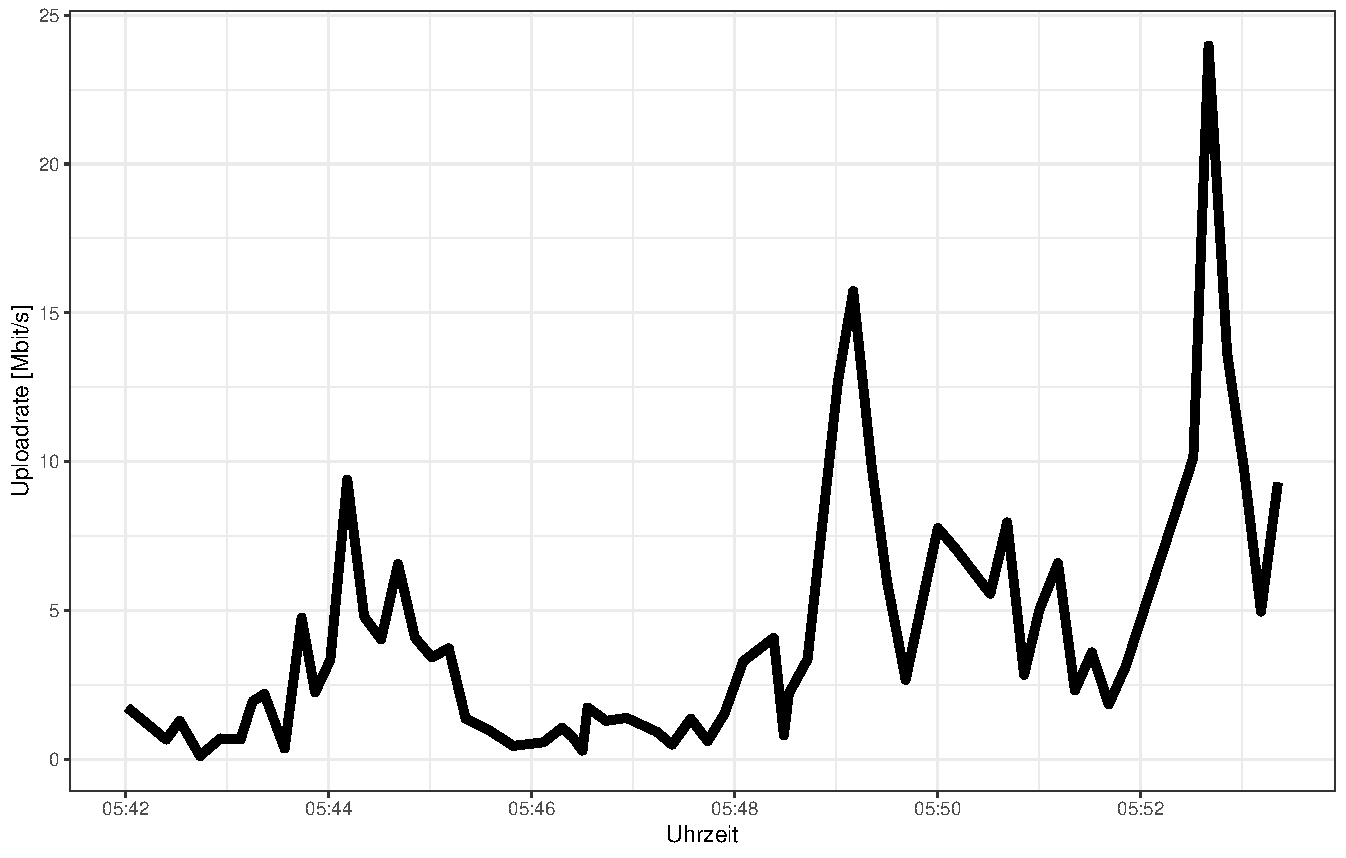
\includegraphics[width=0.8\textwidth]{abbildungen/highway_drive_vodafone}
    \caption{Die erste Messfahrt auf der Autobahn f\"ur den Netzbetreiber Vodafone am 12.12.2018.}
    \label{fig:messfahrt-vodafone}
\end{figure}

In Abbildung~\ref{fig:validierung} ist die in diesem Projekt eingesetzte Validierungsmethode einmal schematisch dargestellt.
Wie bereits beschrieben, besteht der gesamte Datensatz an Messungen f\"ur einen Netzbetreiber aus zehn einzelnen Messfahrten f\"ur
jedes der Szenarien \textit{campus}, \textit{highway}, \textit{suburban} und \textit{urban}.
Jeder dieser Fahrten kann also chronologisch eine Nummer von 1-10 zugewiesen werden, welche zusammen mit dem Szenario
eine Fahrt eindeutig identifiziert.
Im hier eingesetzten Validierungsverfahren wurde nun zun\"achst der gesamte Datensatz in zwei Teile aufgeteilt.
Der erste Teil besteht aus den Fahrten 1-7, der zweite Teil besteht aus den Fahrten 8-10.
In der Trainingsphase und beim Parametertuning kommt ausschlie{\ss}lich der erste Teil der Fahrten 1-7 zum Einsatz.
So wird sichergestellt, dass das Modell beim Training keine Informationen aus zuk\"unftigen Fahrten mit einbeziehen kann, wie
es beispielsweise bei der $k$-fachen Kreuzvalidierung der Fall w\"are. Fahrten 8-10 werden also ausschlie{\ss}lich zur Modellvalidierung
eingesetzt.

\begin{figure}
    \centering
    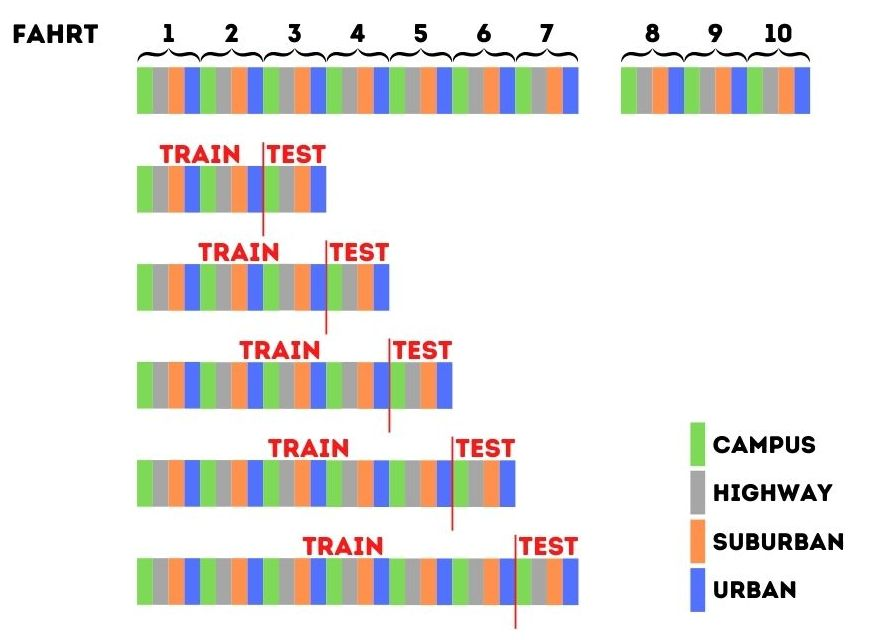
\includegraphics[width=0.8\textwidth]{abbildungen/validierung}
    \caption{Das eingesetzte Verfahren zur Modellvalidierung.}
    \label{fig:validierung}
\end{figure}

\paragraph{Kennzahlen zur Evaluation der Vorhersagequalit\"at}

Um die Vorhersagequalit\"at der eingesetzten Verfahren zu bewerten, werden die Kennzahlen
$R^2$, sowie der Mean Absolute Error (MAE) auf den Out-of-Sample Fahrten 8-10 wie folgt berechnet:
\begin{equation}
    R^2 = 1 - \frac{\sum_{i=1}^n \left( t_i - r_i \right)^2}{\sum_{i=1}^n \left( t_i - \bar{t} \right)^2}
\end{equation}
\begin{equation}
    \text{MAE} = \frac{1}{n} \sum_{i=1}^n \left| t_i - r_i \right|
\end{equation}
Hierbei ist $n$ die Anzahl der vorhergesagten Datenpunkte, $t_i$ gibt den wahren Wert der Zielgr\"o{\ss}e des $i$-ten Datenpunktes an,
$r_i$ gibt den vorhergesagten Wert f\"ur die Zielgr\"o{\ss}e des $i$-ten Datenpunktes an und $\bar{t}$ bezeichnet den Mittelwert der
Zielgr\"o{\ss}e.

\paragraph{Tuning der Hyperparameter}

Das Tuning der Hyperparameter wird systematisch auf den Fahrten 1-7 mithilfe einer zuf\"alligen Gittersuche vorgenommen.
Dabei wird f\"ur jedes Modell ein fester Suchraum der Hyperparameter definiert, welcher entlang jeder Dimension in feste
Gitterpunkte unterteilt wird. Das entstehende Gitter wird dann an einer festen Anzahl zuf\"alliger Stellen ausgewertet
und die zugeh\"origen Parameterkombinationen werden evaluiert.

Zur Evaluation einer Parameterkombination kommt, wie sich in Abbildung~\ref{fig:validierung} ebenfalls
erkennen l\"asst, eine Art Kreuzvalidierung f\"ur Zeitreihen zum Einsatz. Dabei wird der Trainingsdatensatz sukzessive um eine Fahrt
erweitert und es wird immer auf der n\"achsten Fahrt getestet.
Dies soll die Begebenheit simulieren, dass nach und nach neue Messfahrten
vorgenommen werden, die den Gesamtdatensatz Schritt f\"ur Schritt erweitern.

Als G\"utekriterium f\"ur eine getestete Parameterkombination wird der MAE verwendet. Die beste Kombination aus Hyperparametern
wird dann im Anschluss auf dem gesamten Trainingsdatensatz der Fahrten 1-7 zur Modellanpassung genutzt und anschlie{\ss}end
auf den Validierungsfahrten 8-10 evaluiert.

\subsection{Extreme Gradient Boosting}
\label{sec:xgboost}

Extreme Gradient Boosting ist ein Verfahren aus dem Bereich des maschinellen Lernens, welches sich
in den letzten Jahren einer immer gr\"o{\ss}eren Beliebtheit erfreut hat~\cite{XGBoost}.
Die Grundlegende Funktionsweise dieses Verfahrens sei im Folgenden kurz beschrieben.

\subsubsection{Ausgangssituation}

Wir gehen davon aus, dass wir \"uber einen Trainingsdatensatz $\mathcal{D} = \{(\mathbf{x}_i, y_i)\}$
der Gr\"o{\ss}e $\left| \mathcal{D} \right| = n$ verf\"ugen, welcher aus den beobachteten Messungen $\mathbf{x}_i \in \mathbb{R}^m$
und der Zielgr\"o{\ss}e $y_i \in \mathbb{R}$ besteht, deren Wert wir vorhersagen wollen.

Das Ziel des Tree Boosting ist es, den Wert von $y_i$ durch ein Ensemble von Entscheidungsb\"aumen (CART)
vorherzusagen:
\begin{equation}
    \hat{y_i} = \phi(\mathbf{x}_i) =  \sum_{k=1}^K f_k(\mathbf{x}_i), \quad f_k \in \mathcal{F}
\end{equation}
Hierbei ist $\mathcal{F}$ die Klasse der besagten Entscheidungsb\"aume, welche in jedem ihrer $T$ Bl\"atter
einen konstanten Wert vorhersagen: $\mathcal{F} = \{f(\mathbf{x}) = w_{q(x)}\}$, wobei $q: \mathbb{R}^m \rightarrow T$
eine Funktion ist, die der Beobachtung $\mathbf{x}$ eines der $T$ Bl\"atter zuordnet und $w \in \mathbb{R}^T$ der Vektor
der Blattvorhersagen (Gewichte) des Baumes ist.

\subsubsection{Zielfunktion}

Die Zielfunktion, welche w\"ahrend des Trainings zur Anpassung des Modells minimiert wird, setzt sich wie folgt zusammen:
\begin{equation}
    \mathcal{L}(\phi) = \sum_{i=1}^n l(\hat{y}_i, y_i) + \sum_{k=1}^K \Omega(f_k)
\end{equation}
Hierbei ist $l$ eine differenzierbare und konvexe Verlustfunktion, welche Aufschluss \"uber die G\"ute der Vorhersage $\hat{y}_i$
liefert. Ein Beispiel ist der quadratische Fehler, welcher durch $l(\hat{y}_i, y_i) = (\hat{y}_i - y_i)^2$ gegeben ist.
Die Funktion $\Omega$ ist ein sogenannter Regularisierungs- oder Strafterm und ist wie folgt definiert:
\begin{equation}
    \Omega(f) = \gamma T + \frac{1}{2} \lambda \left \lVert w \right \rVert^2
\end{equation}
Das Ziel von $\Omega$ ist es, eine zu hohe Komplexit\"at der einzelnen Entscheidungsb\"aume in der Optimierung zu bestrafen und somit
w\"ahrend des Trainings simplere B\"aume zu bevorzugen. Dies geschieht mit dem Hintergedanken, eine \"Uberanpassung des Modells an
die Trainingsdaten verhindern zu wollen.
Der Parameter $\gamma$ bestraft hierbei die Anzahl der Bl\"atter $T$ eines Entscheidungsbaumes und der Parameter $\lambda$ bestraft
zu gro{\ss}e Gewichte in den einzelnen Bl\"attern.

\subsubsection{Training}

Das Grundprinzip des Boosting ist es, die Ensemble Modelle additiv nach dem Greedy-Prinzip zu trainieren.
Dies funktioniert hier so, dass die einzelnen Entscheidungsb\"aume nicht alle gleichzeitig angepasst werden, sondern
nach und nach zum Ensemble hinzugef\"ugt werden. Jeder Baum, welcher in einem Schritt hinzugef\"ugt wird, wird so trainiert,
dass er die Zielfunktion soweit wie m\"oglich minimiert.

Wenn im Optimierungsschritt $t$ also der Entscheidungsbaum $f_t$ zum Ensemble hinzugef\"ugt wird, ergibt sich die folgende
Verlustfunktion, welche durch $f_t$ minimiert werden soll:
\begin{equation}
    \mathcal{L}^{(t)} = \sum_{i=1}^n l(\hat{y}^{(t-1)}_i + f_t(\mathbf{x}_i), y_i) + \Omega(f_t)
\end{equation}
Die Regularisierungsterme $\sum_{k=1}^{t-1} \Omega(f_k)$ der bereits zum Ensemble hinzugef\"ugten B\"aume wurden hierbei weggelassen,
da sie im Zuge der Optimierung in Schritt $t$ nicht mehr ver\"andert werden k\"onnen.

Beim Extreme Gradient Boosting wird $\mathcal{L}^{(t)}$ nun im Punkt $\hat{y}^{(t-1)}_i$ durch ein Taylor-Polynom 2. Grades
approximiert, welches sich analytisch minimieren l\"asst.
Streicht man alle konstanten Terme, welche f\"ur die Minimierung keine Rolle spielen, erh\"alt man so die folgende Taylor-Approximation:
\begin{equation}
    \tilde{\mathcal{L}}^{(t)} = \sum_{i=1}^{n} \left[ g_i f_t(x_i) + \frac{1}{2}h_i f_t^2(x_i) \right] + \Omega(f_t)
\end{equation}
Hierbei sind $g_i = \partial_{\hat{y}_i^{(t-1)}} l(y_i, \hat{y}_i^{(t-1)})$ und 
$h_i = \partial_{\hat{y}_i^{(t-1)}}^2 l(y_i, \hat{y}_i^{(t-1)})$ die erste und zweite partielle Arbleitung der Verlustfunktion
$l$.

Wie in~\cite{XGBoost} gezeigt wurde, lassen sich dann die optimalen Gewichte $w_j^*, j=1 \ldots T$ f\"ur eine gegebene Baumstruktur
$q$ durch analytische Minimierung von $\tilde{\mathcal{L}}^{(t)}$ berechnen.
Die Bestimmung einer optimalen Baumstruktur $q$ hingegen ist rechnerisch durch Enumeration aller erdenklichen M\"oglichkeiten im
Normalfall keine Option.
Daher wird analog zum CART-Algorithms ein Greedy-Verfahren eingesetzt, welches den Baum durch sukzessives Hinzuf\"ugen neuer
Verzweigungen aufbaut.
Jede neue Verzweigung wird dabei so gew\"ahlt, dass der Wert von $\tilde{\mathcal{L}}^{(t)}$ durch die Bestimmung der optimalen
Gewichte zum aktuellen Baum soweit wie m\"oglich minimiert wird.
Der Regularisierungsterm $\Omega(f_t)$ verhindert dabei direkt durch seine Anwesenheit in $\tilde{\mathcal{L}}^{(t)}$, dass die neue
Baumstruktur zu komplex wird.

\subsubsection{Hyperparameter}

Die Hyperparameter des Extreme Gradient Boosting, welche im Rahmen dieses Projektes durch Tuning
ermittelt wurden, seien im Folgenden kurz aufgelistet:
\begin{itemize}
    \item $n$: Anzahl der Boosting-Runden und damit auch Anzahl der B\"aume, die insgesamt zum Ensemble hinzugef\"ugt werden.
        Je gr\"o{\ss}er dieser Parameter gew\"ahlt wird, desto komplexer wird das Modell.
    \item $\gamma$: Regularisierungsterm, welcher die Anzahl an Bl\"attern eines Entscheidungsbaumes bestraft.
        Dies soll die Bildung von zu komplexen B\"aumen im Ensemble verhindern und somit eine Ma{\ss}nahme gegen potenzielle
        \"Uberanpassung sein.
    \item $\lambda$: Bestraft zu hohe Gewichte in den Bl\"attern eines Entscheidungsbaumes, wird ebenfalls zur Vermeidung von
        \"Uberanpassung verwendet.
    \item $\eta$: Wurde in einer Boosting-Runde ein neuer Baum gefunden, so geht er nur mit dem Gewicht $\eta$ in das 
        Gesamtensemble ein. Dies ist eine weitere Ma{\ss}nahme, die gegen \"Uberanpassung des Modells helfen soll.
\end{itemize}
Der Suchraum, welcher im Tuningprozess zur Ermittlung einer m\"oglichst guten Kombination der Hyperparameter verwendet wurde, 
sei ebenfalls hier angegeben:
\begin{itemize}
    \item $n \in \left[100, 1000 \right]$
    \item $\gamma \in \left[0, 10 \right]$
    \item $\lambda \in \left[0, 10 \right]$
    \item $\eta \in \left[0.01, 1 \right]$
\end{itemize}

\subsection{Lineare Regression mit ARMA-Fehlern}
\label{sec:arma}
